\vspace{0.5cm}

\section*{Descripción e Idea}

\noindent Así como en el episodio $20$ de la cuarta temporada del show \textit{The Big Bang Theory} se muestra a los rumores (coloquialmente conocidos como \textbf{chismes}) como un "Lubricante social en comunidades" - Amy, modelaremos a los rumores como un autómata celular. \\


\noindent Este autómata constaría de los $2$ estados ya conocidos $\{ 0,1 \}$ añadiendo un estado extra, el "amarillo del semáforo" un estado de suceptibilidad a transmitir o dejar morir el chisme. Este estado sería probabilistico, y el nivel de suceptibilidad dependería de un parámetro dado por el usuario, a este parámetro le llamaremos "la sasón" limitado entre $3$ niveles, el más bajo para un chisme poco interesante y el más alto para un buen chisme (chisme jugoso). Obviamente cada uno de los rangos no será totalitario en el conjunto de suceptibles, se tendrán diferentes porcentajes preestipulados para tener siempre suceptibles pertenecientes a las $3$ opciones. Todo esto tiene su nivel de irrealismo y subjetivilidad, pero eso le da su propio gusto a este proyecto.



\section*{Procedimiento/Trabajo a Realizar}

\noindent Investigar hacerca de la teoria de autómatas celulares, tipos de vecindades\footnote{Donde $d$ se refiere a la dimensión del autómata y $k$ al rango de la vecindad.} (Von Neumann $V(d)$, Moore $M(d,k)$, etc.), Modelo de Nagel-Schreckenberg\footnote{(Na-Sch) Modelo del flujo de tránsito con un autómata celular probabilístico.}, cadenas de Markov, se utilizará la bibliografía ya encontrada más lo que poco a poco se consiga. Decidir el lenguaje de programación que se adapte mejor a lo que se busca con este proyecto, a priori sería \textit{Python}, \textit{Mathematica} o algún otro lenguaje (como \textit{Fortran}) acompañado con \textit{Gnuplot}. 


\section*{Ejemplo}

Tomando un estado inicial dado por la siguiente matriz:

$$
\left(
\begin{array}{cccccc}
 0 & 0 & 0.5 & 0.4 & 0.8 & 0.4 \\
 0.5 & 0.8 & 0.4 & 0.6 & 0 & 0 \\
 0 & 0 & 0 & 1 & 0 & 0 \\
 0 & 0.5 & 0.9 & 0.1 & 0 & 0.4 \\
 0 & 0.4 & 0.8 & 0.5 & 0 & 0 \\
 0 & 0.4 & 0.9 & 0.4 & 0.6 & 0 \\
\end{array}
\right)
$$

Se tendría, visualmente, tal que así (Utilizando la función \texttt{ArrayPlot[]})

\begin{figure}[H]
	\centering
	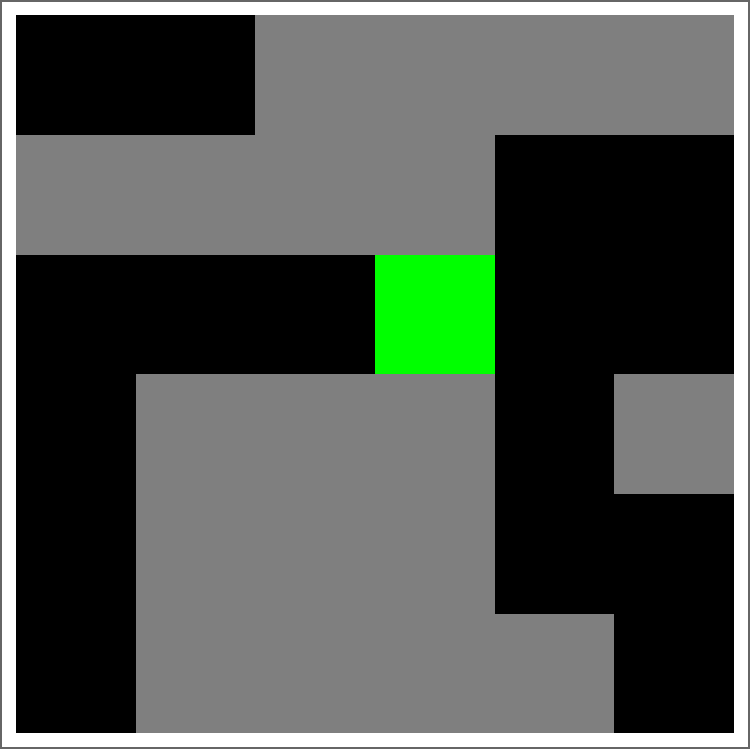
\includegraphics[scale=0.5]{./img/array.pdf}
	\caption{Estado inicial de un chisme, conocedores (células verdes), suceptibles (células grises) y no interesados (células negras).}
\end{figure}




\section*{Extras}
En caso de lograr lo anteriormente mencionado, podría ampliarse el proyecto a realizar esta idea con más colores, o llevandola al 3D. Obviamente, en 3 dimensiones ya no tendría sentido la idea del chisme...o si?


%%%%